\documentclass[border=15pt, tikz]{standalone}
\usepackage[T1]{fontenc}
\usepackage[utf8]{inputenc}
\usepackage{tikz}
\usetikzlibrary{positioning, arrows.meta, decorations.pathreplacing, calc, fit}
\definecolor{clrattention}{HTML}{45B7D1}
\definecolor{clrattention_alt}{HTML}{96E6F0}
\definecolor{clrffn}{HTML}{F97068}
\definecolor{clrnorm}{HTML}{FFD93D}
\definecolor{clrembed}{HTML}{6BCB77}
\definecolor{clrresidual}{HTML}{4D96FF}
\definecolor{clroutput}{HTML}{C084FC}
\definecolor{clrspectral}{HTML}{22D3EE}
\definecolor{clrphysics}{HTML}{FB923C}
\definecolor{clrborder}{HTML}{334155}
\definecolor{clrtext}{HTML}{1E293B}
\definecolor{clrgroup_frame}{HTML}{94A3B8}
\definecolor{clrgroup_fill}{HTML}{F1F5F9}
\begin{document}
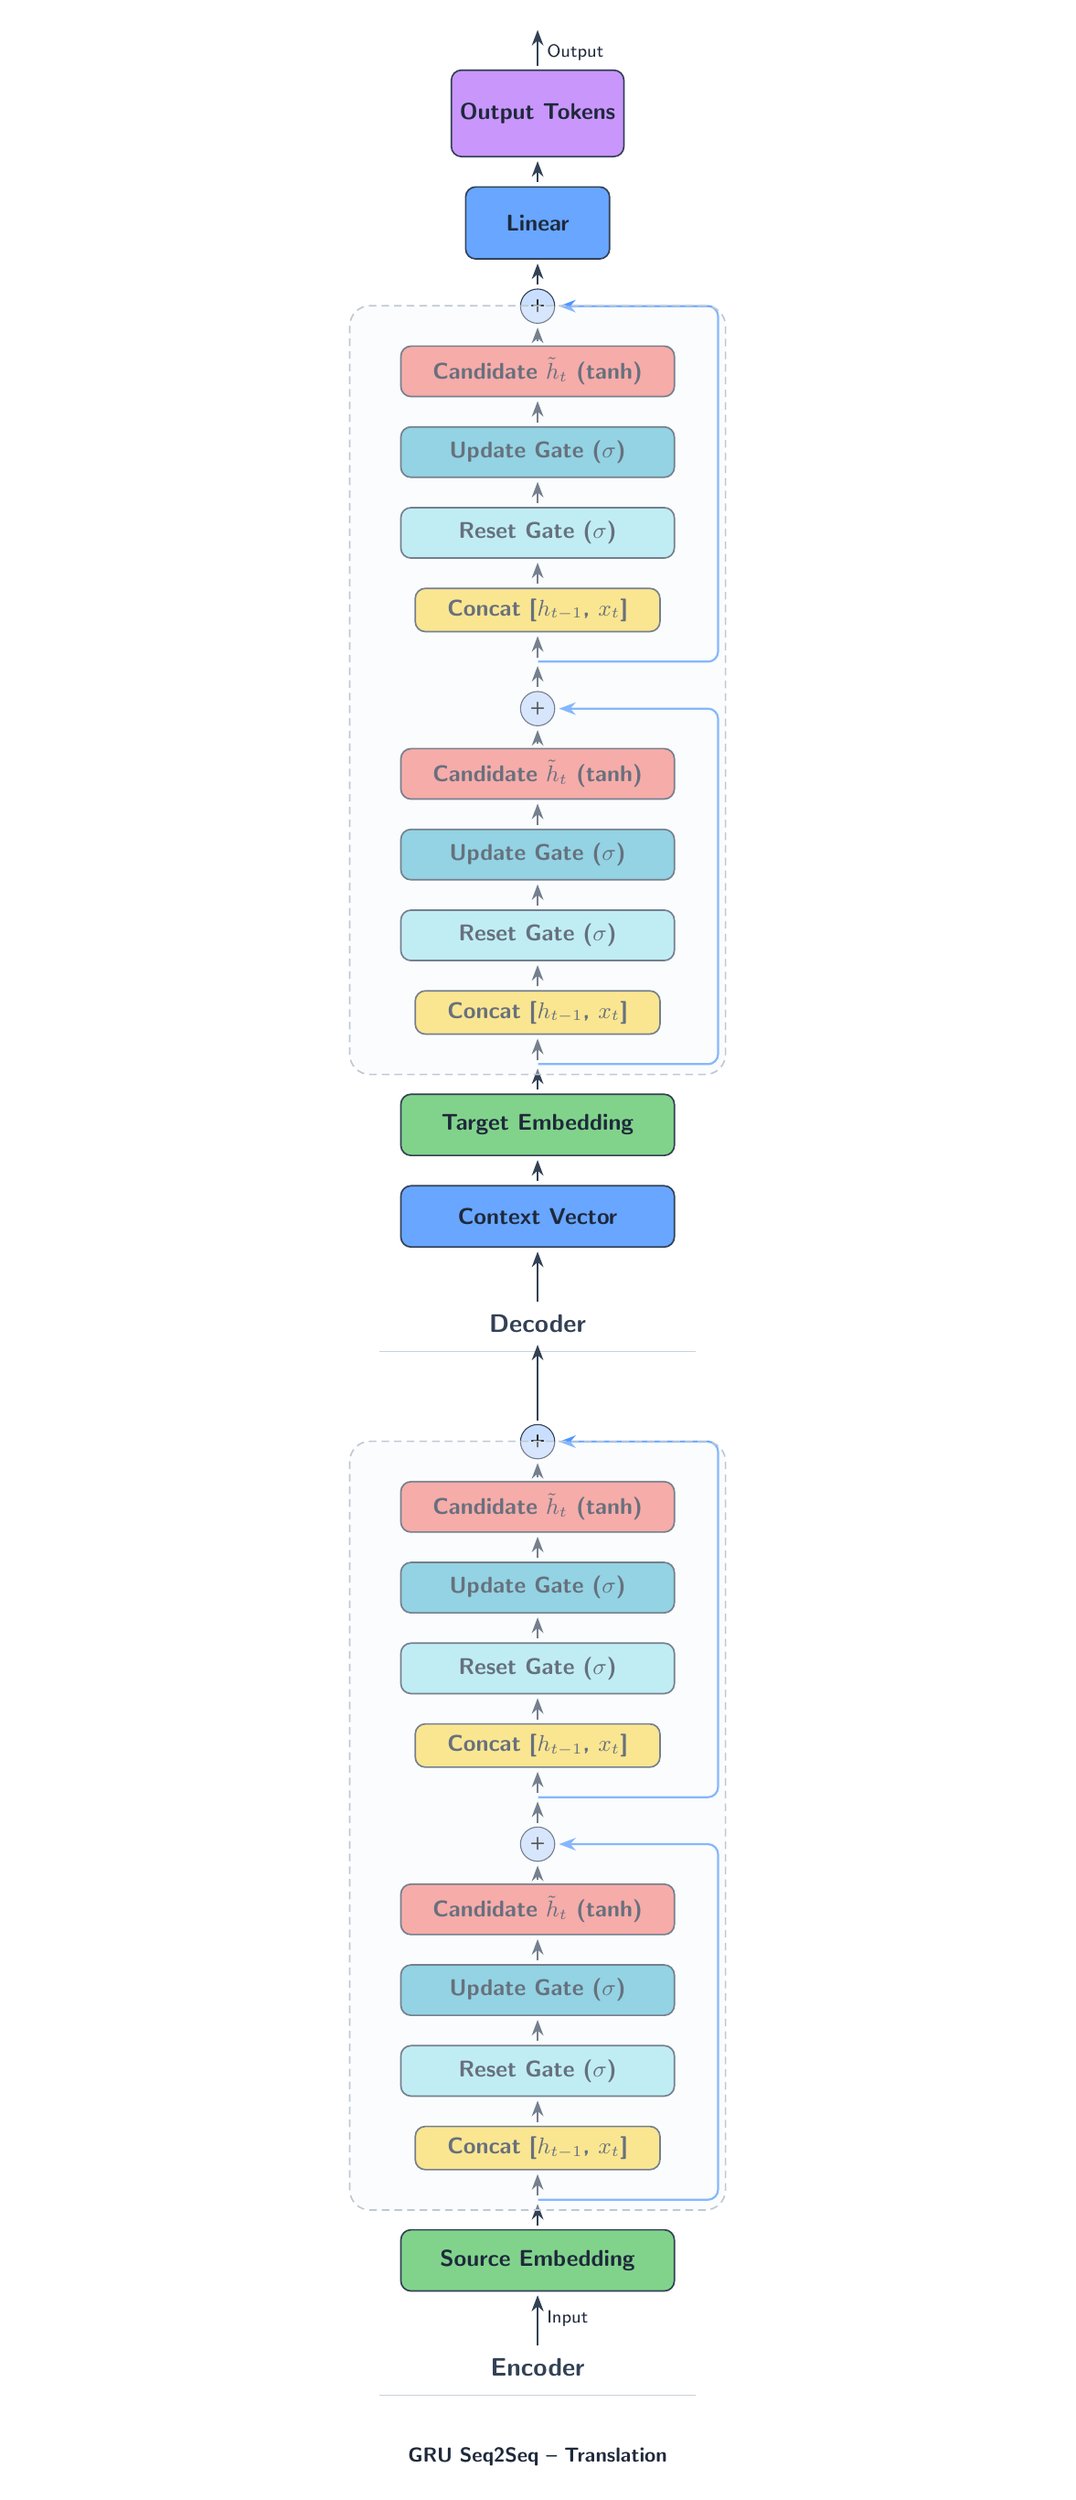
\begin{tikzpicture}[
    >=Stealth,
    every node/.style={font=\sffamily},
    block/.style={draw=clrborder, rounded corners=4pt, minimum width=3.8cm,
                  minimum height=0.85cm, font=\sffamily\small\bfseries,
                  text=clrtext, line width=0.6pt},
    arrow/.style={->, thick, color=clrborder, line width=0.7pt, shorten >=1.5pt, shorten <=1.5pt},
    skiparrow/.style={->, thick, color=clrresidual, line width=0.8pt, rounded corners=4pt, shorten >=1.5pt},
    label/.style={font=\sffamily\scriptsize, text=clrtext},
    subtitle/.style={font=\sffamily\footnotesize, text=clrtext},
]
\node[inner sep=0, minimum height=0] (n_1_rule) at (0,0) {};
\draw[color=clrgroup_frame!50, line width=0.4pt] ([xshift=-2.2cm]n_1_rule.center) -- ([xshift=2.2cm]n_1_rule.center);
\node[above=4pt of n_1_rule, font=\sffamily\normalsize\bfseries, text=clrborder] (n_1) {Encoder};
\node[block, fill=clrembed!85, minimum width=3.8cm, minimum height=0.85cm, text=clrtext, above=0.8cm of n_1] (n_2) {Source Embedding};
\node[inner sep=0, minimum size=0, above=0.4cm of n_2] (res_entry_3) {};
\node[block, fill=clrnorm!85, minimum width=3.4cm, minimum height=0.6cm, text=clrtext, above=0.4cm of res_entry_3] (n_4) {Concat [$h_{t-1}$, $x_t$]};
\node[block, fill=clrattention_alt!85, minimum width=3.8cm, minimum height=0.7cm, text=clrtext, above=0.4cm of n_4] (n_5) {Reset Gate ($\sigma$)};
\node[block, fill=clrattention!85, minimum width=3.8cm, minimum height=0.7cm, text=clrtext, above=0.4cm of n_5] (n_6) {Update Gate ($\sigma$)};
\node[block, fill=clrffn!85, minimum width=3.8cm, minimum height=0.7cm, text=clrtext, above=0.4cm of n_6] (n_7) {Candidate $\tilde{h}_t$ (tanh)};
\node[circle, draw=clrborder, fill=clrresidual!30, inner sep=2pt, font=\sffamily\scriptsize\bfseries, above=0.3cm of n_7] (add_8) {+};
\node[inner sep=0, minimum size=0, above=0.4cm of add_8] (res_entry_9) {};
\node[block, fill=clrnorm!85, minimum width=3.4cm, minimum height=0.6cm, text=clrtext, above=0.4cm of res_entry_9] (n_10) {Concat [$h_{t-1}$, $x_t$]};
\node[block, fill=clrattention_alt!85, minimum width=3.8cm, minimum height=0.7cm, text=clrtext, above=0.4cm of n_10] (n_11) {Reset Gate ($\sigma$)};
\node[block, fill=clrattention!85, minimum width=3.8cm, minimum height=0.7cm, text=clrtext, above=0.4cm of n_11] (n_12) {Update Gate ($\sigma$)};
\node[block, fill=clrffn!85, minimum width=3.8cm, minimum height=0.7cm, text=clrtext, above=0.4cm of n_12] (n_13) {Candidate $\tilde{h}_t$ (tanh)};
\node[circle, draw=clrborder, fill=clrresidual!30, inner sep=2pt, font=\sffamily\scriptsize\bfseries, above=0.3cm of n_13] (add_14) {+};
\node[inner sep=0, minimum height=0, above=1.0cm of add_14] (n_15_rule) {};
\draw[color=clrgroup_frame!50, line width=0.4pt] ([xshift=-2.2cm]n_15_rule.center) -- ([xshift=2.2cm]n_15_rule.center);
\node[above=4pt of n_15_rule, font=\sffamily\normalsize\bfseries, text=clrborder] (n_15) {Decoder};
\node[block, fill=clrresidual!85, minimum width=3.8cm, minimum height=0.85cm, text=clrtext, above=0.8cm of n_15] (n_16) {Context Vector};
\node[block, fill=clrembed!85, minimum width=3.8cm, minimum height=0.85cm, text=clrtext, above=0.4cm of n_16] (n_17) {Target Embedding};
\node[inner sep=0, minimum size=0, above=0.4cm of n_17] (res_entry_18) {};
\node[block, fill=clrnorm!85, minimum width=3.4cm, minimum height=0.6cm, text=clrtext, above=0.4cm of res_entry_18] (n_19) {Concat [$h_{t-1}$, $x_t$]};
\node[block, fill=clrattention_alt!85, minimum width=3.8cm, minimum height=0.7cm, text=clrtext, above=0.4cm of n_19] (n_20) {Reset Gate ($\sigma$)};
\node[block, fill=clrattention!85, minimum width=3.8cm, minimum height=0.7cm, text=clrtext, above=0.4cm of n_20] (n_21) {Update Gate ($\sigma$)};
\node[block, fill=clrffn!85, minimum width=3.8cm, minimum height=0.7cm, text=clrtext, above=0.4cm of n_21] (n_22) {Candidate $\tilde{h}_t$ (tanh)};
\node[circle, draw=clrborder, fill=clrresidual!30, inner sep=2pt, font=\sffamily\scriptsize\bfseries, above=0.3cm of n_22] (add_23) {+};
\node[inner sep=0, minimum size=0, above=0.4cm of add_23] (res_entry_24) {};
\node[block, fill=clrnorm!85, minimum width=3.4cm, minimum height=0.6cm, text=clrtext, above=0.4cm of res_entry_24] (n_25) {Concat [$h_{t-1}$, $x_t$]};
\node[block, fill=clrattention_alt!85, minimum width=3.8cm, minimum height=0.7cm, text=clrtext, above=0.4cm of n_25] (n_26) {Reset Gate ($\sigma$)};
\node[block, fill=clrattention!85, minimum width=3.8cm, minimum height=0.7cm, text=clrtext, above=0.4cm of n_26] (n_27) {Update Gate ($\sigma$)};
\node[block, fill=clrffn!85, minimum width=3.8cm, minimum height=0.7cm, text=clrtext, above=0.4cm of n_27] (n_28) {Candidate $\tilde{h}_t$ (tanh)};
\node[circle, draw=clrborder, fill=clrresidual!30, inner sep=2pt, font=\sffamily\scriptsize\bfseries, above=0.3cm of n_28] (add_29) {+};
\node[block, fill=clrresidual!85, minimum width=2.0cm, minimum height=1.0cm, text=clrtext, above=0.4cm of add_29] (n_30) {Linear};
\node[block, fill=clroutput!85, minimum width=2.0cm, minimum height=1.2cm, text=clrtext, above=0.4cm of n_30] (n_31) {Output Tokens};
\draw[arrow] (n_1.north) -- (n_2.south);
\draw[arrow] (n_4.north) -- (n_5.south);
\draw[arrow] (n_5.north) -- (n_6.south);
\draw[arrow] (n_6.north) -- (n_7.south);
\draw[arrow] (res_entry_3.north) -- (n_4.south);
\draw[arrow] (n_7.north) -- (add_8.south);
\draw[skiparrow] (res_entry_3.east) -- ++(2.5,0) |- (add_8.east);
\draw[arrow] (n_2.north) -- (res_entry_3.south);
\draw[arrow] (n_10.north) -- (n_11.south);
\draw[arrow] (n_11.north) -- (n_12.south);
\draw[arrow] (n_12.north) -- (n_13.south);
\draw[arrow] (res_entry_9.north) -- (n_10.south);
\draw[arrow] (n_13.north) -- (add_14.south);
\draw[skiparrow] (res_entry_9.east) -- ++(2.5,0) |- (add_14.east);
\draw[arrow] (add_8.north) -- (res_entry_9.south);
\draw[arrow] (add_14.north) -- (n_15.south);
\draw[arrow] (n_15.north) -- (n_16.south);
\draw[arrow] (n_16.north) -- (n_17.south);
\draw[arrow] (n_19.north) -- (n_20.south);
\draw[arrow] (n_20.north) -- (n_21.south);
\draw[arrow] (n_21.north) -- (n_22.south);
\draw[arrow] (res_entry_18.north) -- (n_19.south);
\draw[arrow] (n_22.north) -- (add_23.south);
\draw[skiparrow] (res_entry_18.east) -- ++(2.5,0) |- (add_23.east);
\draw[arrow] (n_17.north) -- (res_entry_18.south);
\draw[arrow] (n_25.north) -- (n_26.south);
\draw[arrow] (n_26.north) -- (n_27.south);
\draw[arrow] (n_27.north) -- (n_28.south);
\draw[arrow] (res_entry_24.north) -- (n_25.south);
\draw[arrow] (n_28.north) -- (add_29.south);
\draw[skiparrow] (res_entry_24.east) -- ++(2.5,0) |- (add_29.east);
\draw[arrow] (add_23.north) -- (res_entry_24.south);
\draw[arrow] (add_29.north) -- (n_30.south);
\draw[arrow] (n_30.north) -- (n_31.south);
\draw[arrow] ([yshift=-0.6cm]n_2.south) -- node[right, yshift=-2pt, font=\sffamily\scriptsize, text=clrtext] {Input} (n_2.south);
\draw[arrow] (n_31.north) -- node[right, yshift=-2pt, font=\sffamily\scriptsize, text=clrtext] {Output} ([yshift=0.6cm]n_31.north);
\node[draw=clrgroup_frame!60, rounded corners=8pt, densely dashed, line width=0.6pt, fill=clrgroup_fill, fill opacity=0.35, inner ysep=0.55cm, inner xsep=0.7cm, fit=(n_4) (n_5) (n_6) (n_7) (n_10) (n_11) (n_12) (n_13)] (g_0) {};
\node[draw=clrgroup_frame!60, rounded corners=8pt, densely dashed, line width=0.6pt, fill=clrgroup_fill, fill opacity=0.35, inner ysep=0.55cm, inner xsep=0.7cm, fit=(n_19) (n_20) (n_21) (n_22) (n_25) (n_26) (n_27) (n_28)] (g_1) {};
\node[below=0.6cm of current bounding box.south, subtitle, text width=14cm, align=center] {\textbf{GRU Seq2Seq -- Translation}};
\end{tikzpicture}
\end{document}
